\documentclass[runningheads]{llncs}
% clear && fastfetch && latexmk -pdf --auxdir="out" main.tex

\usepackage{amsmath}
\usepackage[T1]{fontenc}
\usepackage{graphicx}
\usepackage{booktabs}   
\usepackage{tikz}       
\usetikzlibrary{positioning,arrows.meta,fit}
\usepackage{cite} 
\usepackage{hyperref}
\usepackage{color}
\renewcommand\UrlFont{\color{blue}\rmfamily}
\urlstyle{rm}


% Inline literal query syntax
\newcommand{\q}[1]{\texttt{\small #1}}
% temporal operator
\newcommand{\tchain}{>{}>}



\begin{document}
% \title{CLIMB at the Video Browser Showdown 2027}
\title{CLIMB at VBS 2027: Multi-Signal Keyframe Retrieval with Collaborative Ad-Hoc Search}
\titlerunning{CLIMB at VBS 2027}
\author{
    Tobias Wurzer\inst{1}\orcidID{0009-0002-0965-6877} \and
    Sebastian Eisner\inst{1} \and
    Klaus Schöffmann\inst{1}\orcidID{0000-0002-9218-1704}
}

% First names are abbreviated in the running head.
% If there are more than two authors, 'et al.' is used.
\authorrunning{T. Wurzer et al.}

\institute{University of Klagenfurt, 9020 Klagenfurt, Austria}
\maketitle



\begin{abstract}
We present CLIMB, an interactive video retrieval system built for the Video Browser Showdown 2027.
Because a single visual embedding often lacks the precision needed to capture fine-grained cues like 
signage, or spoken dialogue, CLIMB retrieves information across four complementary signals: 
visual embeddings, on-screen text, generated captions, and speech transcripts.
By combining rank-based fusion with a hybrid of lexical and semantic matching, the system ensures broad retrieval coverage.
Additionally, queries can be chained into temporal sequences, providing increased flexibility while significantly narrowing the results set.
For ad-hoc video search, CLIMB treats retrieval as a shared team activity by automatically hiding teammate-submitted shots from all active results. 
Crucially, core functions like search, browsing, and submission remain fully operational even if the shared session service becomes unreachable.

\keywords{
  Video Browser Showdown  \and 
  Interactive Video Retrieval \and 
  Collaborative Search \and 
  Semantic Embedding.
}
\end{abstract}



\section{Introduction}
The Video Browser Showdown~\cite{vbsoverview} is an interactive video retrieval competition asking participants 
to solve known-item search (KIS), ad-hoc video search (AVS), and visual question-answering (VQA/QAS) tasks 
against large scale video collections. For VBS 2027, the main collection is V3C~\cite{v3c} with 28{,}450 videos, 
roughly 3{,}800 hours, and about 4.7\,TB, segmented into 4.14 million master shots, 
alongside the smaller MVK~\cite{mvk} and GynSurgLHE~\cite{GynSurgLHE} collections.

Successfully addressing these tasks presents two fundamental challenges. First, a single visual embedding is often 
too vague to capture precise task hints, such as specific on-screen text or spoken dialogue. 
Second, because AVS scoring rewards distinct correct shots, a team of $n$ operators searching independently
spends a substantial share of its submissions re-finding what a teammate has already sent.

CLIMB addresses both. It indexes every video as scenes and keyframes, retrieves over four independent signals, 
fuses them by rank, and treats an AVS task as a single shared activity rather than $n$ parallel ones, vanishing 
uplicate scenes from everybody's list. 
Concretely, we contribute:
\begin{enumerate}
    \item Keyframe-level retrieval fusing four heterogeneous signals by rank (Sect.~\ref{fusion}).
    \item A temporal query language, \q{A \tchain{} B \tchain{}(120) C}, in which every stage is itself a full query (Sect.~\ref{chains}).
    \item A collaborative, network-resilient AVS mode (Sect.~\ref{avs}).
    \item An index engineered for everyday hardware: binary-quantized HNSW with oversample-and-rerank (Sect.~\ref{pipeline}).
\end{enumerate}


\section{System Overview}
CLIMB is built from six components (Fig.~\ref{architecture}). Decoding each video, segmenting it into scenes, 
selecting keyframes, computing embeddings, reading text on screen, as well as captioning and transcribing, 
happens in an offline pipeline described in Sect.~\ref{pipeline}. The resulting scenes, keyframes, 
and four indexes that get queried by the retrievers land in a PostgreSQL database.

At query time, the system runs as two processes, a Node.js backend handling media, DRES communication, and the AVS mirror 
and a Python engine handling models, query embedding and rank fusion. Both connect to the database: the backend reads metadata directly,
delegating only search execution to Python. The frontend (Sect.~\ref{search}), communicates exclusively with the Node.js backend.

For scenarios where network reliability is a concern, CLIMB supports fully localized deployments, serving media asstes directly from localhost. 
Additionally the shared and optional AVS session service (Sect.~\ref{avs}) only transmits a few kilobytes of JSON polled every four seconds.




\begin{figure}[t]
  \centering
  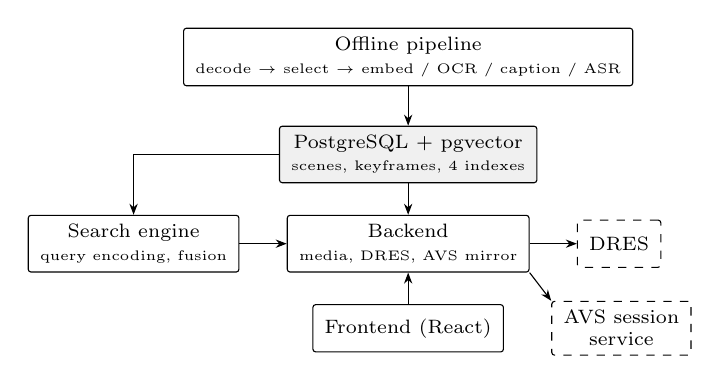
\begin{tikzpicture}[
   % https://www.underleaf.ai/learn/tikz/block-diagrams
    box/.style={draw, rounded corners=1pt, align=center,
                font=\scriptsize, minimum height=6mm, inner xsep=1.5mm},
    store/.style={box, fill=black!6},
    ext/.style={box, dashed, fill=white},
    flow/.style={-{Stealth[length=1.4mm]}, thin}
  ]
    \node[box]                    (pipe) {Offline pipeline\\{\tiny decode $\to$ select $\to$ embed / OCR / caption / ASR}};
    \node[store, below=5mm of pipe] (db) {PostgreSQL + pgvector\\{\tiny scenes, keyframes, 4 indexes}};
    \node[box,   below=4mm of db]  (be) {Backend\\{\tiny media, DRES, AVS mirror}};
    \node[box,   left=6mm of be]    (se) {Search engine\\{\tiny query encoding, fusion}};
    \node[box,   below=4mm of be]   (fe) {Frontend (React)};
    \node[ext,   right=6mm of be] (dres) {DRES};
    \node[ext,   right=6mm of fe]  (avs) {AVS session\\service};

    \draw[flow] (pipe) -- (db);
    \draw[flow] (db)   -- (be);
    \draw[flow] (db.west) -| (se.north);
    \draw[flow] (se)   -- (be);
    \draw[flow] (fe)   -- (be);
    \draw[flow] (be)   -- (dres);
    \draw[flow] (be.south east) -- (avs.north west);
  \end{tikzpicture}
  \caption{
    CLIMB architecture. All components can run locally on each machine, except for two external services: 
    DRES and the AVS session service, which is deployed once.
  }
  \label{architecture}
\end{figure}



\section{Indexing Pipeline} \label{pipeline}
\subsection{Scenes and Keyframe Selection}
The V3C dataset provides scene boundaries. These scene boundaries are the center of our encoding. They get used, splitting 
the video into different scenes. For each of these scenes, we select between 2 and 32 keyframes according to the length of the scene,
selecting one keyframe per four seconds.

We start by selecting the most typical frame and then repeatedly add the frame, which is most different from the already
selected keyframes. This selects a broad coverage of keyframes. Afterward we 
reject frames, that are nearly flat and have almost no edges.
This reduced the number of keyframes sampled from our subset (Sect.~\ref{results}) from 99.661 keyframes
at 1 fps to 35{,}558 keyframes. Damaged bitstreams are indexed from what we were able to decode, flagged, and logged. 


\subsection{Feature Extraction}
CLIMB extracts four signals per scene, ensuring a divers set of retrieval possiblities. They are deliberately not applied equally. 
Two keyframe-, two scene-based. OCR is of the first type, leveraging the 
PP-OCR \cite{ppocr3} model, and for embedding a visual representation into a 1024-dimensional vector space, we use SigLIP2 \cite{siglip2}. 

Given the high computational cost and intra-scene visual redundancy, captioning is restricted to each scene's first keyframe. 
For full-scale captioning we intend to leverage Qwen2-VL-2B-Instruct \cite{qwen}, but used the lightweight SmolVLM-256M-Instruct \cite{smolvlm} for testing. 
Audio transcription is handled by Whisper \cite{whisper}.

In order to encode textual signals into semantic embeddings, we use multilingual-e-base \cite{e5base}, 
embedding into a 768-dimensional vector space. 
For efficient retrieval, all generated embeddings are stored using an HNSW index \cite{hnsw} 
over binary-quantized vectors. To maintain search accuracy while minimizing memory overhead, initial search candidates are reranked against their full-precision vectors. 
This quantization significantly reduces the memory footprint, requiring only 5.3\,GB for 12.4M keyframes compared to 28\,GB for half-precision storage.


\section{Retrieval Model}
\subsection{Rank-Based Fusion at Keyframe Level} \label{fusion}
As discussed before, we use four different encoders to encode as broad a spectrum of information as possible, 
but the signals do not produce comparable scores on their own. 
A small 20-query test on our subset returns a score of $0.17$ for the best visual result (due to the modality gap described in \cite{modalityGap}), 
whilst the best caption match was a $0.93$. In order to avoid sensitive and model specific calibration we use a ranked based fusion approch, explaine below.

Each signal returns a list of ranked objects. Whilst the visual signal and 
OCR signal natively return a list of ranked keyframes, the caption and audio signals are scene-based. 
Thus, each keyframe inherits the rank of its parent scene.
The keyframes are then merged via weighted Reciprocal Rank Fusion (RRF) \cite{rrf}. This works similarly to normal RRF but weighs the 
signals depending on their source, allowing us to highlight keyframes found via specific encoders, i.e., 
OCR, where a lexical hit is much more likely to belong to the correct scene than a similar visual embedding. 
The fused ranking score for a keyframe $d \in D$ is defined as:
\begin{equation}
RRFscore(d \in D) = \sum_{r \in R}\frac{w(r)}{60 + r(d)}
\end{equation}
where $r(d)$ is the rank assigned by encoder $r \in R$ with weight $w(r)$ \cite{rrf}.

\subsection{Semantic and Lexical matching}
While cross-modal visual retrieval with SigLIP2 is inherently semantic, the remaining text-to-text signals could theoretically rely on lexical matching.
However, strict keyword matching on generated captions suffers from severe vocabulary mismatch. For instance, a query for "law enforcement" shares zero lexical 
overlap with a highly relevant caption describing "a police uniform" In fact, the terms "law" and "enforcement" never appear within our extracted captions. 

While ASR transcripts are embedded semantically for conceptual and cross-lingual search, users can invoke a "said:" operator for exact lexical matching of specific quotes.
Conversely, OCR operates as a purely lexical signal to pinpoint exact on-screen text provided in task hints. Semantic matching here is redundant, as general concepts are already captured by the visual embedding.

\subsection{Query Language and Temporal Chains} \label{chains}
Some retrieval tasks require describing not a single scene, but a temporally ordered sequence of scenes, such as a bridge followed by a beach.
A plain text query searches all four signals at once, and the operator prefixes in Table ~\ref{tabSyntax} restrict it to a single source, 
whilst \q{\tchain{}} joins queries into ordered temporal chains. 

The chaining makes the prefixes much more powerful. A query \q{A \tchain{} B \tchain{} C} is 3 stages, 
where each one is a complete query on its own. \q{text: pegasus \tchain{} mountain bike race} finds a scene with a text that reads "pegasus", 
followed by a scene that matches with mountain bike race, independent of a single encoder. 
An unannotated chain searches for scenes in the same video that are at maximum 60 seconds apart, annotated with \q{(120)} or \q{(d120)}; it's 120 seconds.
The maximum delta is ten minutes, with up to four stages per chain.

\begin{table}[t]
  \caption{
    Query syntax. Prefixes restrict searches to specific signals, while \q{\tchain{}} chains queries temporally within a single video.
  }
  \label{tabSyntax}
  \centering 
  \begin{tabular}{@{}ll@{}}
    \toprule
    Input & Effect \\
    \midrule
    \q{a drawing of people on a beach}            & Global search (all signals) \\
    \q{text: state capitol}                       & On-screen text only \\
    \q{said: new york}                            & Spoken audio only \\
    \q{-video:00191}                              & Exclude a video (repeatable) \\
    \q{a video game sunset \tchain{} door}        & Sequential search (same video) \\
    \bottomrule
  \end{tabular}
\end{table}
% ---
\section{Interactive Search} \label{search}
\subsection{The Search Loop} \label{loop}
A search typically follows an iterative interaction loop. The operator enters a query, which returns a grid of keyframes. Selecting one, 
displays a five-second scene preview starting at the corresponding timestamp. The filmstrip located under the video player,
provides an overview of all the keyframes allowing for efficient navigation between them. Keyframe times get populated automatically but remain editable, 
to fine-tune the target submission frame.
Additionally, there is a variety of button based controls for quick search refinement. 
To keep this cycle responsive, query results are cached and paginated: the initial query executes the search, 
while subsequent pages are loaded from cache upon scrolling.
\emph{Submit to DRES} sends the selected timestamp. \emph{Exclude video from search} removes a video from the results and 
when textual queries fall short, \emph{Find Similar} enables visual query-by-example. 
Finally, dedicated UI inputs support VQA tasks, allowing operators to submit text-only or combined text-and-shot answers.


\begin{figure}[t]
\centering
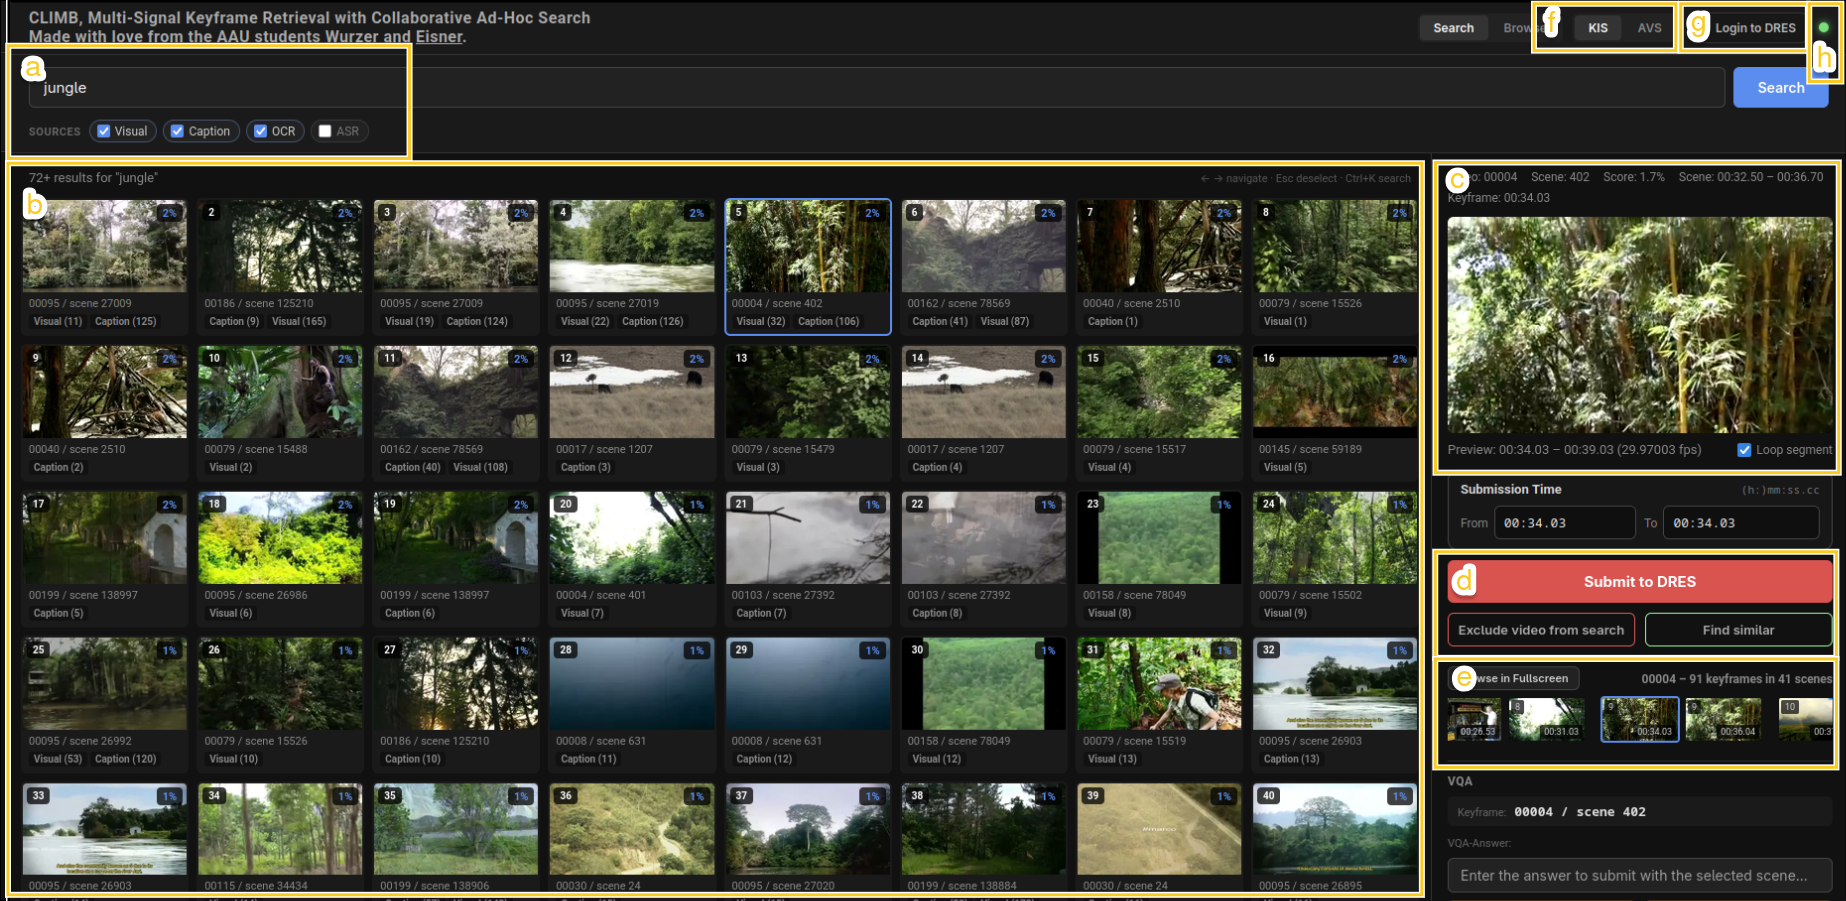
\includegraphics[width=\textwidth]{figures/ui-screenshot-annoted.png}
\caption{
  The CLIMB interface:
  (a) query bar and source filters,
  (b) scene result grid,
  (c) detail panel and video player,
  (d) submission and search-refinement controls,
  (e) keyframe filmstrip,
  (f) AVS session tab,
  (g) DRES connection controls, and
  (h) system health status.
}
\label{ui}
\end{figure}


\subsection{Submitting to DRES}
As with every browser at VBS, the DRES-Submission pipeline is an integral part of CLIMB \cite{dres,dres2}. 
The login dialog accepts a \emph{server URL}, \emph{evaluation name}, and \emph{credentials}. If the requested evaluation is missing, CLIMB alerts and falls back.
When submitting, each request returns a status, consisting of a status code, summary, and verdict. 
Correct submissions are indicated in green, pending ones in yellow, and incorrect or rejected ones in red.

AVS submissions follow go through additional steps, as described in Sect.~\ref{avs}. 
From the operator's perspective, however, the interaction is analogous to that of a default KIS task.
After switching to the AVS tab in the top-right corner of the interface and joining a session, 
submissions can be made through the same interaction pattern. 
The primary difference is that accepted submissions are hidden from other participants in the same session.


\section{Collaborative Ad-Hoc Video Search} \label{avs}
Since AVS scoring rewards distinct correct shots, independently searching team members tend to identify the same
obvious results first, resulting in a large fraction of duplicate submissions. 
We address this problem by making an AVS session a shared state. Submitted scenes are consequently hidden 
from the results of all session participants. Other scenes in these videos get marked as covered, 
but not hidden to promote a diverse submission set, whilst allowing for submission of multiple distinct scenes from 
the same video. 

Importantly, search and submissions do not depend on the speed or availability of the AVS collaboration service. To ensure this separation, 
CLIMB sends the submission request to the DRES server before attempting to communicate with the, independently deployed, collaboration service.


\section{Preliminary Results} \label{results}
While implemented for the full V3C collection, our reported metrics were measured on a 200-video subset (25\,h, 14{,}345 shots, 35{,}558 keyframes).

Compared with exhaustive exact search (108\,ms), oversampling 1{,}000 candidates before exact reranking recovers 15 of the 
true top 20 in 29\,ms, 2{,}000 candidates recover 18 in 54\,ms, and 4{,}000 all 20 in 91\,ms. The reamining discrepancy is due to the binary quantization
rather than the index: the ANN stage ranks by Hamming distance over 1-bit vectors. CLIMB defaults to 1{,}000 candidates, while keeping this parameter configurable.

Although a far simpler CLIMB prototype won our university's course-internal retrieval competition, VBS presents a much greater challenge. 
Our latency measurements are limited to a small subset rather than the full-scale collection, and neither MVK nor GynSurg resembles the imagery SigLIP2 was trained on.


\section{Conclusion}
We presented CLIMB, an interactive video retrieval system for VBS 2027. It uses rank-based fusion to combine visual embeddings, 
on-screen text, generated captions, and transcripts at the keyframe level, while supporting temporally chained queries. 
% A collaborative mode hides teammate-submitted shots and degrades gracefully, keeping core search functions fully available offline.
A collaborative mode hides shots a teammate already submitted from everyone's results while search, browsing and submission remain unaffected when the shared session service is unavailable.

Our next steps include completing ingestion of the full collection and addressing the domain gap for MVK and GynSurg, where the 
general-purpose visual embeddings of SigLIP2 are expected to be least effective.


%\begin{credits}
%\subsubsection{\ackname} A bold run-in heading in small font size at the end of the paper is
%used for general acknowledgments, for example: This study was funded
%by X (grant number Y).

%\subsubsection{\discintname}
%It is now necessary to declare any competing interests or to specifically
%state that the authors have no competing interests. Please place the
%statement with a bold run-in heading in small font size beneath the
%(optional) acknowledgments\footnote{If EquinOCS, our proceedings submission
%system, is used, then the disclaimer can be provided directly in the system.},
%for example: The authors have no competing interests to declare that are
%relevant to the content of this article. Or: Author A has received research
%grants from Company W. Author B has received a speaker honorarium from
%Company X and owns stock in Company Y. Author C is a member of committee Z.
%\end{credits}


% ---- Bibliography ----
% BibTeX users should specify bibliography style 'splncs04'.
% References will then be sorted and formatted in the correct style.
\bibliographystyle{splncs04}
\bibliography{climb}

\end{document}
